% 原书印刷72--79页，PDF物理99--106页，止于2.5标题之前.
\subsection{作为二次最优运输极限的Knothe运输}\label{sec:2.4}

稍微修改\autoref{sec:1.3.1}讨论的二次成本，将其替换为加权二次成本
\[
c_\varepsilon(x,y):=\sum_{i=1}^d\lambda_i(\varepsilon)(x_i-y_i)^2,
\]
其中$\lambda_i(\varepsilon)$是依赖于参数$\varepsilon>0$的正标量. 若$\mu$关于Lebesgue测度绝对连续，相应的最优运输问题就有唯一解$\mathrm T_\varepsilon$. 为简单起见，本节只考虑$\mu$与$\nu$的支集紧的情形（但一切都能调整到$\int|x|^2\,d\mu,\int|y|^2\,d\nu<+\infty$的情形）.

若还满足：对所有$k\in\{1,\ldots,d-1\}$，当$\varepsilon\to0$时，$\lambda_k(\varepsilon)/\lambda_{k+1}(\varepsilon)\to0$，则自然会预期$\mathrm T_\varepsilon$收敛到Knothe运输$\mathrm T$. Y.~Brenier曾猜想这一收敛结果，认为它十分自然.

我们将在上一节的绝对连续性假设下证明它. 另一方面，\cite{b114}在稍弱的假设下证明了同一结果，即要求所有分解后的测度无原子. 有趣之处在于，也需要目标测度$\nu$无原子；若不满足这一条件，便存在不收敛的反例.

\begin{example}[Gauss测度的显式计算]\label{obj:2.22}
为在有显式解的特殊情形中说明问题，取$d=2$，并取两个Gauss测度$\mu=N(0,\mathrm I)$与
$\nu=N\!\left(0,\begin{pmatrix}a&b\\b&c\end{pmatrix}\right)$，其中$ac>b^2$、$a>0$；记号$N(a,A)$表示以$a$为中心、协方差矩阵为$A$的Gauss密度. 取$\lambda_1(\varepsilon)=\varepsilon$、$\lambda_2(\varepsilon)=1$. 可以验证（另见\autoref{ex:11}），$\mathrm T_\varepsilon$为线性映射，且其在$\mathbb R^2$标准基下的矩阵为
\[
\mathrm T_\varepsilon=
\frac{1}{\sqrt{a\varepsilon^2+c+2\varepsilon\sqrt{ac-b^2}}}
\begin{pmatrix}
a\varepsilon+\sqrt{ac-b^2}&b\\
b\varepsilon&c+\varepsilon\sqrt{ac-b^2}
\end{pmatrix}.
\]
当$\varepsilon\to0$时，它收敛到
\[
\mathrm T=\begin{pmatrix}\sqrt{a-b^2/c}&b/\sqrt c\\0&\sqrt c\end{pmatrix},
\]
即从$\mu$到$\nu$的Knothe运输的矩阵.
\end{example}

直接陈述第一个结果；其证明具有$\Gamma$-收敛展开的精神（见\cite{b77}和\autoref{box:4.6}），需要分几步完成.

\begin{theorem}\label{obj:2.23}\index{0004@$\Gamma$-收敛（$\Gamma$-convergence）!005@高阶展开（higher order developments）|hyperpage}
设$\mu$与$\nu$是$\mathbb R^d$上两个紧支撑的绝对连续概率测度，且$\gamma_\varepsilon\in\Pi(\mu,\nu)$为成本
$c_\varepsilon(x,y)=\sum_{i=1}^d\lambda_i(\varepsilon)(x_i-y_i)^2$的最优运输方案，其中权重$\lambda_k(\varepsilon)>0$. 假设对每个$k\in\{1,\ldots,d-1\}$，当$\varepsilon\to0$时有$\lambda_k(\varepsilon)/\lambda_{k+1}(\varepsilon)\to0$. 设$\mathrm T$为$\mu$与$\nu$之间的Knothe--Rosenblatt映射，$\gamma_K\in\mathscr P(\mathbb R^d\times\mathbb R^d)$为相应的运输方案（即$\gamma_K:=(\mathrm{id},\mathrm T)_\#\mu$）. 则当$\varepsilon\to0$时，$\gamma_\varepsilon\rightharpoonup\gamma_K$.

此外，方案$\gamma_\varepsilon$由运输映射$\mathrm T_\varepsilon$诱导，且当$\varepsilon\to0$时，这些映射在$L^2(\mu)$中收敛到$\mathrm T$.
\end{theorem}

证明大致遵循以下策略. 取$\gamma_\varepsilon$的一个极限点，证明它与$\gamma_K$具有相同的$(x_d,y_d)$边缘测度. 然后关于$(x_d,y_d)$分解，证明条件$(x_{d-1},y_{d-1})$边缘测度一致. 反复使用这一论证，就能完成证明.

\begin{proof}
不失一般性，假设$\lambda_d(\varepsilon)=1$且$\lambda_i(\varepsilon)/\lambda_{i+1}(\varepsilon)\to0$.

取最优方案$\gamma_\varepsilon$，假设$\gamma_\varepsilon\rightharpoonup\gamma$（取子列即可做到）. 要证明$\gamma=\gamma_K$. 由Knothe运输的唯一性，收敛将对整个序列成立，而不仅对子列成立.

将$\gamma_\varepsilon$与$\gamma_K$比较，并使用最优性，首先得到
\begin{equation}\label{eq:2.5}
\int c_\varepsilon\,d\gamma_\varepsilon\le\int c_\varepsilon\,d\gamma_K.
\end{equation}
由于$c_\varepsilon$一致收敛到$c^{(d)}(x,y)=(x_d-y_d)^2$（将使用一般记号$c^{(k)}(x,y)=|x_k-y_k|^2$），令$\varepsilon\to0$便得到
\[
\int c^{(d)}\,d\gamma\le\int c^{(d)}\,d\gamma_K.
\]
而函数$c^{(d)}$只依赖于变量$x_d$、$y_d$，所以上式表明，对于二次成本，测度$(\pi_d^{x,y})_\#\gamma$的结果至少与$(\pi_d^{x,y})_\#\gamma_K$一样好（$\pi_d^{x,y}$为$x$与$y$的最后坐标上的投影，即$\pi_d^{x,y}(x,y)=(x_d,y_d)$）. 然而，选择测度$\gamma_K$时，正是要使它对于这一成本在$\mu^d$与$\nu^d$之间最优，而且该最优运输方案唯一. 因而$(\pi_d^{x,y})_\#\gamma=(\pi_d^{x,y})_\#\gamma_K$. 将这一共同测度记为$\gamma^d$.

回到\eqref{eq:2.5}，注意所有测度$\gamma_\varepsilon$与$\gamma_K$具有相同的边缘测度，故它们分别在$x_d$与$y_d$上的投影为$\mu^d$与$\nu^d$. 这意味着，对一维二次成本，$(\pi_d^{x,y})_\#\gamma_\varepsilon$的结果不可能优于$(\pi_d^{x,y})_\#\gamma_K$. 因此
\[
\begin{aligned}
&\int|x_d-y_d|^2\,d(\pi_d^{x,y})_\#\gamma_K(x_d,y_d)
 +\sum_{i=1}^{d-1}\lambda_i(\varepsilon)\int(x_i-y_i)^2\,d\gamma_\varepsilon\\
&\quad\le\int c_\varepsilon\,d\gamma_\varepsilon\le\int c_\varepsilon\,d\gamma_K\\
&\quad=\int|x_d-y_d|^2\,d(\pi_d^{x,y})_\#\gamma_K(x_d,y_d)
 +\sum_{i=1}^{d-1}\lambda_i(\varepsilon)\int(x_i-y_i)^2\,d\gamma_K.
\end{aligned}
\]
消去公共项，除以$\lambda_{d-1}(\varepsilon)$并取极限，得到
\begin{equation}\label{eq:2.6}
\int c^{(d-1)}\,d\gamma\le\int c^{(d-1)}\,d\gamma_K.
\end{equation}
注意这两个积分都只依赖于$x_{d-1}$与$y_{d-1}$. 不过，可以投影到变量$(x_{d-1},x_d)$与$(y_{d-1},y_d)$上（得到测度$(\pi_{d-1,d}^{x,y})_\#\gamma$与$(\pi_{d-1,d}^{x,y})_\#\gamma_K$），从而关于测度$\gamma^d$进行分解. 有
\begin{equation}\label{eq:2.7}
\begin{aligned}
&\int d\gamma^d(x_d,y_d)\int|x_{d-1}-y_{d-1}|^2\,d\gamma^{d-1}_{(x_d,y_d)}(x_{d-1},y_{d-1})\\
&\qquad\le\int d\gamma^d(x_d,y_d)\int|x_{d-1}-y_{d-1}|^2\,d\gamma^{d-1}_{(x_d,y_d),K}(x_{d-1},y_{d-1}).
\end{aligned}
\end{equation}
要证明测度$\gamma^{d-1}_{(x_d,y_d)}$在$x_{d-1}$与$y_{d-1}$上的边缘测度，与相应的$\gamma^{d-1}_{(x_d,y_d),K}$相同. 若能如此，则前者的二次成本不会优于相应的$\gamma^{d-1}_{(x_d,y_d),K}$的成本（因为选择Knothe测度时，正是要使固定$x_d$与$y_d$后，关于$(x_{d-1},y_{d-1})$的二次成本最优）. 而\eqref{eq:2.7}表明，平均而言，这些测度给出的结果不劣于最优测度的结果. 因此，对几乎每对$(x_d,y_d)$，两个结果相同；由一维最优运输的唯一性，得到$\gamma^{d-1}_{(x_d,y_d)}=\gamma^{d-1}_{(x_d,y_d),K}$. 为使这一证明成立，只需对$\gamma^d$-几乎每对$(x_d,y_d)$证明两个测度的边缘测度相同. 对固定的$(x_d,y_d)$，希望证明，对任意$\varphi$，有
\[
\int\varphi(x_{d-1})\,d\gamma^{d-1}_{(x_d,y_d)}
=\int\varphi(x_{d-1})\,d\gamma^{d-1}_{(x_d,y_d),K}
\]
（并对$y_{d-1}$的函数证明类似等式）. 因为要对几乎每对$(x_d,y_d)$证明它，只需对任意$\varphi$与$\psi$证明
\[
\begin{aligned}
&\int d\gamma^d(x_d,y_d)\,\psi(x_d,y_d)\int\varphi(x_{d-1})\,d\gamma^{d-1}_{(x_d,y_d)}\\
&\qquad=\int d\gamma^d(x_d,y_d)\,\psi(x_d,y_d)\int\varphi(x_{d-1})\,d\gamma^{d-1}_{(x_d,y_d),K}.
\end{aligned}
\]
也就是证明
\[
\int\psi(x_d,y_d)\varphi(x_{d-1})\,d\gamma^{d-1}
=\int\psi(x_d,y_d)\varphi(x_{d-1})\,d\gamma_K^{d-1},
\]
这并不平凡. 到目前为止，只知道两个测度$\gamma^{d-1}$与$\gamma_K^{d-1}$关于$(x_{d-1},x_d)$、$(y_{d-1},y_d)$的边缘测度相同（因为它们在$x$与$y$上的投影相同），关于$(x_d,y_d)$的边缘测度也相同（刚刚已证明）. 但这里出现了三个变量$(x_{d-1},x_d,y_d)$的函数. 然而，已知测度$\gamma^d$集中于某个映射$\mathrm T^d$的集合$y_d=\mathrm T^d(x_d)$上（这里用到了最优方案确实来自映射），因此可替换$y_d$的表达式，消去一个变量. 这说明函数$\psi(x_d,y_d)\varphi(x_{d-1})$实际只依赖于$(x_{d-1},x_d)$，从$\gamma$换成$\gamma_K$时等式便成立. 对函数$\psi(x_d,y_d)\varphi(y_{d-1})$可作相同处理，但此时必须保证能将$x_d$替换为$y_d$的函数，也就是$\mathrm T^d$可逆. 由$\nu^d$的绝对连续性，这是可能的：$\mathrm T^d$是从$\mu^d$到$\nu^d$的最优运输，反方向也存在最优运输，而且由于唯一性，它给出同一个最优方案. 这些事实证明测度$\gamma^{d-1}_{(x_d,y_d)}$与$\gamma^{d-1}_{(x_d,y_d),K}$具有相同的边缘测度，因此，由于它们都最优，对几乎每对$(x_d,y_d)$都相同. 这蕴含$(\pi_{d-1,d}^{x,y})_\#\gamma=(\pi_{d-1,d}^{x,y})_\#\gamma_K$；将这一共同测度记为$\gamma^{d-1}$.

若$d=2$，证明已经完成. 现在可以如下继续归纳：对$N$归纳证明，当$d\le N$时定理成立；并且无论维数是多少，对每个$k\ge d-(N-1)$，都有$(\pi_{k,d}^{x,y})_\#\gamma=(\pi_{k,d}^{x,y})_\#\gamma_K$（即第$k$至第$d$个分量收敛）. 这两点在$N=2$时均已证明.

假设结果对某个$N$成立. 取$d>N$与$k=d-(N-1)$. 要证明$(\pi_{k-1,d}^{x,y})_\#\gamma=(\pi_{k-1,d}^{x,y})_\#\gamma_K$. 若能做到，证明就完成了，因为这也说明结果在$d=N+1$维时成立（此时$k=2$，再做这一步便完成证明）.

写成$x=(x^-,x^+)$与$y=(y^-,y^+)$，其中$x^-,y^-\in\mathbb R^{k-1}$，$x^+,y^+\in\mathbb R^{d-k+1}$（分成截至第$k-1$个分量和从第$k$个开始的分量）. 定义一个竞争方案$\gamma_K^\varepsilon$如下：$\gamma_K^\varepsilon$是$\mathbb R^d\times\mathbb R^d$上的测度，具有边缘测度
\[
(\pi_{x^-,x^+})_\#\gamma_K^\varepsilon=\mu,\qquad
(\pi_{y^-,y^+})_\#\gamma_K^\varepsilon=\nu,\qquad
(\pi_{x^+,y^+})_\#\gamma_K^\varepsilon=\eta_{\varepsilon,k},
\]
其中$\eta_{\varepsilon,k}$是在边缘测度$\mu^k=(\pi_{x^+})_\#\mu$与$\nu^k=(\pi_{y^+})_\#\nu$之间，使运输成本$\sum_{i=k}^d\lambda_i(\varepsilon)c^{(i)}$最优的测度. 由证明的递归结构，已知$\eta_{\varepsilon,k}$收敛到$(\pi_{x^+,y^+})_\#\gamma_K$（因为假设结果在$N$维成立）.

还需要说明如何构造测度$\gamma_K^\varepsilon$（它很可能不唯一）. 一个简单方法如下：分别按$\pi_{x^+}$与$\pi_{y^+}$分解$\mu$与$\nu$，得到两族测度$\mu^{x^+}$与$\nu^{y^+}$. 对每对$(x^+,y^+)$，取它们之间的一个运输方案$\gamma^{x^+,y^+}$. 测度$\gamma^{x^+,y^+}\otimes\eta_{\varepsilon,k}$就满足所需性质. 此外，将$\gamma^{x^+,y^+}$选为这两个测度之间的Knothe运输. 事实上，对证明的这一步，唯一重要的是关于第$k-1$个分量，对任意$(x^+,y^+)$，选择从$\mu_{k-1}^{x^+}:=(\pi_{x_{k-1}})_\#\mu^{x^+}$到$\nu_{k-1}^{y^+}:=(\pi_{y_{k-1}})_\#\nu^{y^+}$的单调映射，使
$\int c^{(k-1)}\,d\gamma^{x^+,y^+}=\mathscr T_c(\mu_{k-1}^{x^+},\nu_{k-1}^{y^+})$（最后这一表达式中的$\mathscr T_c$表示实直线上的二次运输成本）.

采用这一选择，写出
\[
\begin{aligned}
&\sum_{i\ge h}\lambda_i(\varepsilon)\int|x_i-y_i|^2\,d\gamma_K^\varepsilon
+\sum_{i=1}^{k-1}\lambda_i(\varepsilon)\int(x_i-y_i)^2\,d\gamma_\varepsilon\\
&\quad\le\int c_\varepsilon\,d\gamma_\varepsilon\le\int c_\varepsilon\,d\gamma_K^\varepsilon\\
&\quad=\sum_{i\ge h}\lambda_i(\varepsilon)\int|x_i-y_i|^2\,d\gamma_K^\varepsilon
+\sum_{i=1}^{k-1}\lambda_i(\varepsilon)\int(x_i-y_i)^2\,d\gamma_K^\varepsilon.
\end{aligned}
\]
因此，消去公共项并除以$\lambda_{k-1}(\varepsilon)$，得到
\[
\int c^{(k-1)}\,d\gamma_\varepsilon
\le\int c^{(k-1)}\,d\gamma_K^\varepsilon
=\int\mathscr T_c(\mu_{k-1}^{x^+},\nu_{k-1}^{y^+})\,d\eta_{\varepsilon,h}.
\]
然后令$\varepsilon\to0$. 最后一个不等式的左边趋于$\int c^{(k-1)}\,d\gamma$，右边则收敛到
\[
\int\mathscr T_c(\mu_{k-1}^{x^+},\nu_{k-1}^{y^+})\,d(\pi_{x^+,y^+})_\#\gamma_K
=\int c^{(k-1)}\,d\gamma_K.
\]
这一收敛由下面从\autoref{obj:1.8}导出的\autoref{obj:2.24}保证. 最终得到
\[
\int c^{(k-1)}\,d\gamma\le\int c^{(k-1)}\,d\gamma_K,
\]
于是可以继续. 得到最后这个不等式的过程与得到\eqref{eq:2.6}的过程类似，但需要更多工作，因为$\gamma_K$并不像$k=d$时那样，对所有$i\ge k$的分量都恰好最优.

关于$\pi_{k,d}^{x,y}$分解，再完全照前面处理：证明分解所得测度的边缘测度相同，就足以证明测度相等. 这里使用如下形式的测试函数：
\[
\psi(x_h,x_{k+1},\ldots,x_d,y_h,y_{k+1},\ldots,y_d)\varphi(x_{k-1})
\]
与
\[
\psi(x_h,x_{k+1},\ldots,x_d,y_h,y_{k+1},\ldots,y_d)\varphi(y_{k-1}).
\]
仍可使用前面的技巧，即用变量$x$的函数替换变量$y$. 要反过来用$y$替换$x$，则需对Knothe运输的一部分求逆. 这是可能的，因为如前所述，我们的假设蕴含所得到的全部单调运输都可逆. 最后与前面一样，得到$\gamma^{k-1}=\gamma_K^{k-1}$. 这说明归纳能从第$N$步推进到第$N+1$步，从而完成证明.

现在已经证明$\gamma_\varepsilon\rightharpoonup\gamma_K$. 而当所有这些运输方案均来自运输映射时，$(\mathrm{id},\mathrm T_\varepsilon)_\#\mu\rightharpoonup(\mathrm{id},\mathrm T)_\#\mu$蕴含$\mathrm T_\varepsilon\to\mathrm T$于$L^2(\mu)$（见下面的\autoref{obj:2.25}）.
\end{proof}

证明中使用了以下结果，它是\autoref{obj:1.8}的推论.

\begin{corollary}\label{obj:2.24}
若$\mu$与$\nu$是$\mathbb R^d=\mathbb R^k\times\mathbb R^{d-k}$上两个紧支撑的概率测度，可分解为$\mu=\mu^+\otimes\mu^{x^+}$与$\nu=\nu^+\otimes\nu^{y^+}$，且$c$为连续成本，则泛函
\[
\eta\longmapsto\int\mathscr T_c(\mu^{x^+},\nu^{y^+})\,d\eta(x^+,y^+)
\]
在$\mu^+$与$\nu^+$之间的运输方案上连续.
\end{corollary}
\begin{proof}
只需在如下设置下应用\autoref{obj:1.8}：$X=Y=\mathbb R^k$，$\widetilde X=\widetilde Y=\mathscr P(\Omega)$，其中$\Omega\subset\mathbb R^{d-k}$使$\operatorname{spt}(\mu),\operatorname{spt}(\nu)\subset\mathbb R^k\times\Omega$. 在空间$\mathscr P(\Omega)$上赋予任意将弱收敛度量化、并使其成为可分度量空间的距离（例如，\autoref{sec:5}给出具有这一性质的距离；也可用Banach空间单位球上弱收敛的标准方法构造）. 对于\autoref{obj:1.8}陈述中出现的成本函数，取$(a,b)\mapsto\mathscr T_c(a,b)$，以及$a(x^+):=\mu^{x^+}$、$b(y^+):=\nu^{y^+}$. 由于这一量由$\max|c|$控制（支集紧），很容易选择两个有界函数$f,g$使$\mathscr T_c(a,b)\le f(a)+g(b)$.
\end{proof}

还需要下面这个简单引理.

\begin{lemma}\label{obj:2.25}
给定$\mu\in\mathscr P(X)$与$\nu_n\in\mathscr P(\Omega)$，其中$\Omega\subset\mathbb R^d$为紧集，假设$\gamma_n:=\gamma_{\mathrm T_n}\in\Pi(\mu,\nu_n)$满足$\gamma_n\to\gamma=\gamma_{\mathrm T}$. 则$\mathrm T_n\to\mathrm T$于$L^2(X,\mu)$.
\end{lemma}
\begin{proof}
由于函数$\mathrm T_n$取值于$\Omega$，它们一致有界，取子列后在$L^2(X,\mu)$中有弱极限. 将这一极限记为$S$. 为证明$S=\mathrm T$，取连续函数$\boldsymbol\xi\in C(X;\mathbb R^d)$，考虑极限
\[
\begin{aligned}
\int(\boldsymbol\xi(x)\cdot S(x))\,d\mu(x)
&=\lim_n\int(\boldsymbol\xi(x)\cdot\mathrm T_n(x))\,d\mu(x)\\
&=\lim_n\int(\boldsymbol\xi(x)\cdot y)\,d\gamma_n(x,y)\\
&=\int(\boldsymbol\xi(x)\cdot y)\,d\gamma_{\mathrm T}(x,y)\\
&=\int(\boldsymbol\xi(x)\cdot\mathrm T(x))\,d\mu(x).
\end{aligned}
\]
这证明了$S=\mathrm T$.

为证明强收敛，只需考虑
\[
\int|\mathrm T_n|^2\,d\mu=\int|y|^2\,d\gamma_n
\longrightarrow\int|y|^2\,d\gamma=\int|\mathrm T|^2\,d\mu.
\]
这说明不仅有$L^2$弱收敛，$L^2$范数也收敛. 如同Hilbert空间中的通常论证，这蕴含强收敛.
\end{proof}

注意，上述证明也适用于其他$L^p$空间，而有界性假设（即紧支撑）可以替换为适当的可积性控制.

这里指出，若不考虑二次成本$c_\varepsilon$，而考虑更一般的可分离成本
\[
c_\varepsilon(x,y):=\sum_{i=1}^d\lambda_i(\varepsilon)c_i(x_i-y_i),
\]
其中每个$c_i$都是光滑严格凸函数（具有适当增长），则前面的收敛证明仍适用.

\begin{example}[测度有原子时的反例]\label{obj:2.26}
现在说明一个有趣事实：\autoref{obj:2.23}中的绝对连续性假设不仅对$\mu$必要，对$\nu$也必要（见\autoref{obj:2.21}，以核对这一情形下Knothe映射的定义）. 给出$\mathbb R^2$中一个十分简单的例子，其中$\mu$关于Lebesgue测度绝对连续而$\nu$不然，并说明定理的结论不成立. 在正方形$\Omega:=[-1,1]\times[-1,1]$上，定义$\mu=\frac12\mathbbm1_E\cdot\mathscr L^2$，其中
$E=\{(x_1,x_2)\in[-1,1]\times[-1,1]:x_1x_2<0\}$，所以$\mu$均匀分布在左上与右下象限；另令$\nu=\frac12\mathscr H^1|_S$，其中$S$为线段$[-1,1]\times\{0\}$.

容易计算，Knothe--Rosenblatt映射为
\[
\mathrm T(x):=(2x_1+\operatorname{sign}(x_2)),0)
\]
（事实上，测度$\nu^2$是在$0$处的Dirac质量，故$\mathrm T^2(x)=0$）. 成本为$|x_1-y_1|^2+\varepsilon|x_2-y_2|^2$的任意运输问题的解都是$\mathrm T^0(x):=(x_1,0)$（没有运输能优于这个到$\nu$的支集的投影）. 因此，在此例中，最优运输映射未能趋于Knothe--Rosenblatt映射. 原因在于测度$\nu^2=\delta_0$中的原子（\autoref{fig:2.3}）.
\end{example}

\begin{figure}[htbp]
\centering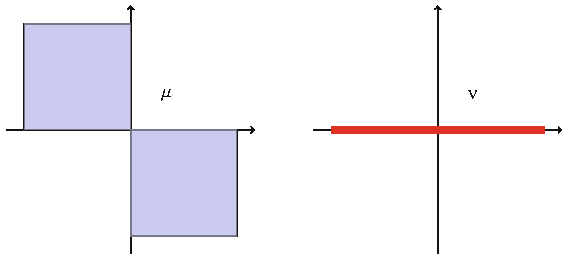
\includegraphics[width=.8\linewidth]{assets/ch02-fig-2-3.pdf}
\caption{反例中的测度$\mu$与$\nu$.}\label{fig:2.3}
\end{figure}
